\documentclass[1p]{elsarticle_modified}
%\bibliographystyle{elsarticle-num}

%\usepackage[colorlinks]{hyperref}
%\usepackage{abbrmath_seonhwa} %\Abb, \Ascr, \Acal ,\Abf, \Afrak
\usepackage{amsfonts}
\usepackage{amssymb}
\usepackage{amsmath}
\usepackage{amsthm}
\usepackage{scalefnt}
\usepackage{amsbsy}
\usepackage{kotex}
\usepackage{caption}
\usepackage{subfig}
\usepackage{color}
\usepackage{graphicx}
\usepackage{xcolor} %% white, black, red, green, blue, cyan, magenta, yellow
\usepackage{float}
\usepackage{setspace}
\usepackage{hyperref}

\usepackage{tikz}
\usetikzlibrary{arrows}

\usepackage{multirow}
\usepackage{array} % fixed length table
\usepackage{hhline}

%%%%%%%%%%%%%%%%%%%%%
\makeatletter
\renewcommand*\env@matrix[1][\arraystretch]{%
	\edef\arraystretch{#1}%
	\hskip -\arraycolsep
	\let\@ifnextchar\new@ifnextchar
	\array{*\c@MaxMatrixCols c}}
\makeatother %https://tex.stackexchange.com/questions/14071/how-can-i-increase-the-line-spacing-in-a-matrix
%%%%%%%%%%%%%%%

\usepackage[normalem]{ulem}

\newcommand{\msout}[1]{\ifmmode\text{\sout{\ensuremath{#1}}}\else\sout{#1}\fi}
%SOURCE: \msout is \stkout macro in https://tex.stackexchange.com/questions/20609/strikeout-in-math-mode

\newcommand{\cancel}[1]{
	\ifmmode
	{\color{red}\msout{#1}}
	\else
	{\color{red}\sout{#1}}
	\fi
}

\newcommand{\add}[1]{
	{\color{blue}\uwave{#1}}
}

\newcommand{\replace}[2]{
	\ifmmode
	{\color{red}\msout{#1}}{\color{blue}\uwave{#2}}
	\else
	{\color{red}\sout{#1}}{\color{blue}\uwave{#2}}
	\fi
}

\newcommand{\Sol}{\mathcal{S}} %segment
\newcommand{\D}{D} %diagram
\newcommand{\A}{\mathcal{A}} %arc


%%%%%%%%%%%%%%%%%%%%%%%%%%%%%5 test

\def\sl{\operatorname{\textup{SL}}(2,\Cbb)}
\def\psl{\operatorname{\textup{PSL}}(2,\Cbb)}
\def\quan{\mkern 1mu \triangleright \mkern 1mu}

\theoremstyle{definition}
\newtheorem{thm}{Theorem}[section]
\newtheorem{prop}[thm]{Proposition}
\newtheorem{lem}[thm]{Lemma}
\newtheorem{ques}[thm]{Question}
\newtheorem{cor}[thm]{Corollary}
\newtheorem{defn}[thm]{Definition}
\newtheorem{exam}[thm]{Example}
\newtheorem{rmk}[thm]{Remark}
\newtheorem{alg}[thm]{Algorithm}

\newcommand{\I}{\sqrt{-1}}
\begin{document}

%\begin{frontmatter}
%
%\title{Boundary parabolic representations of knots up to 8 crossings}
%
%%% Group authors per affiliation:
%\author{Yunhi Cho} 
%\address{Department of Mathematics, University of Seoul, Seoul, Korea}
%\ead{yhcho@uos.ac.kr}
%
%
%\author{Seonhwa Kim} %\fnref{s_kim}}
%\address{Center for Geometry and Physics, Institute for Basic Science, Pohang, 37673, Korea}
%\ead{ryeona17@ibs.re.kr}
%
%\author{Hyuk Kim}
%\address{Department of Mathematical Sciences, Seoul National University, Seoul 08826, Korea}
%\ead{hyukkim@snu.ac.kr}
%
%\author{Seokbeom Yoon}
%\address{Department of Mathematical Sciences, Seoul National University, Seoul, 08826,  Korea}
%\ead{sbyoon15@snu.ac.kr}
%
%\begin{abstract}
%We find all boundary parabolic representation of knots up to 8 crossings.
%
%\end{abstract}
%\begin{keyword}
%    \MSC[2010] 57M25 
%\end{keyword}
%
%\end{frontmatter}

%\linenumbers
%\tableofcontents
%
\newcommand\colored[1]{\textcolor{white}{\rule[-0.35ex]{0.8em}{1.4ex}}\kern-0.8em\color{red} #1}%
%\newcommand\colored[1]{\textcolor{white}{ #1}\kern-2.17ex	\textcolor{white}{ #1}\kern-1.81ex	\textcolor{white}{ #1}\kern-2.15ex\color{red}#1	}

{\Large $\underline{12a_{1246}~(K12a_{1246})}$}

\setlength{\tabcolsep}{10pt}
\renewcommand{\arraystretch}{1.6}
\vspace{1cm}\begin{tabular}{m{100pt}>{\centering\arraybackslash}m{274pt}}
\multirow{5}{120pt}{
	\centering
	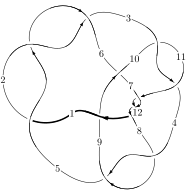
\includegraphics[width=112pt]{../../../GIT/diagram.site/Diagrams/png/2047_12a_1246.png}\\
\ \ \ A knot diagram\footnotemark}&
\allowdisplaybreaks
\textbf{Linearized knot diagam} \\
\cline{2-2}
 &
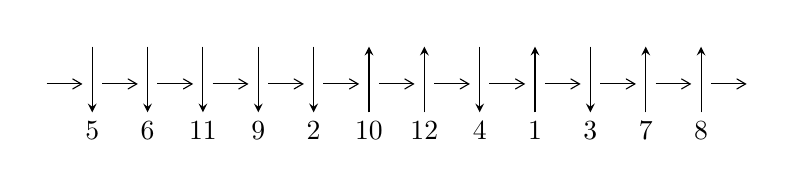
\begin{tikzpicture}[x=20pt, y=17pt]
	% nodes
	\node (C0) at (0, 0) {};
	\node (C1) at (1, 0) {};
	\node (C1U) at (1, +1) {};
	\node (C1D) at (1, -1) {5};

	\node (C2) at (2, 0) {};
	\node (C2U) at (2, +1) {};
	\node (C2D) at (2, -1) {6};

	\node (C3) at (3, 0) {};
	\node (C3U) at (3, +1) {};
	\node (C3D) at (3, -1) {11};

	\node (C4) at (4, 0) {};
	\node (C4U) at (4, +1) {};
	\node (C4D) at (4, -1) {9};

	\node (C5) at (5, 0) {};
	\node (C5U) at (5, +1) {};
	\node (C5D) at (5, -1) {2};

	\node (C6) at (6, 0) {};
	\node (C6U) at (6, +1) {};
	\node (C6D) at (6, -1) {10};

	\node (C7) at (7, 0) {};
	\node (C7U) at (7, +1) {};
	\node (C7D) at (7, -1) {12};

	\node (C8) at (8, 0) {};
	\node (C8U) at (8, +1) {};
	\node (C8D) at (8, -1) {4};

	\node (C9) at (9, 0) {};
	\node (C9U) at (9, +1) {};
	\node (C9D) at (9, -1) {1};

	\node (C10) at (10, 0) {};
	\node (C10U) at (10, +1) {};
	\node (C10D) at (10, -1) {3};

	\node (C11) at (11, 0) {};
	\node (C11U) at (11, +1) {};
	\node (C11D) at (11, -1) {7};

	\node (C12) at (12, 0) {};
	\node (C12U) at (12, +1) {};
	\node (C12D) at (12, -1) {8};
	\node (C13) at (13, 0) {};

	% arrows
	\draw[->,>={angle 60}]
	(C0) edge (C1) (C1) edge (C2) (C2) edge (C3) (C3) edge (C4) (C4) edge (C5) (C5) edge (C6) (C6) edge (C7) (C7) edge (C8) (C8) edge (C9) (C9) edge (C10) (C10) edge (C11) (C11) edge (C12) (C12) edge (C13) ;	\draw[->,>=stealth]
	(C1U) edge (C1D) (C2U) edge (C2D) (C3U) edge (C3D) (C4U) edge (C4D) (C5U) edge (C5D) (C6D) edge (C6U) (C7D) edge (C7U) (C8U) edge (C8D) (C9D) edge (C9U) (C10U) edge (C10D) (C11D) edge (C11U) (C12D) edge (C12U) ;
	\end{tikzpicture} \\
\hhline{~~} \\& 
\textbf{Solving Sequence} \\ \cline{2-2} 
 &
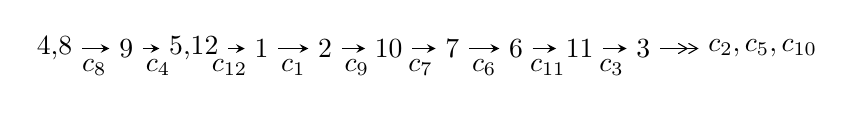
\begin{tikzpicture}[x=23pt, y=7pt]
	% node
	\node (A0) at (-1/8, 0) {4,8};
	\node (A1) at (1, 0) {9};
	\node (A2) at (33/16, 0) {5,12};
	\node (A3) at (25/8, 0) {1};
	\node (A4) at (33/8, 0) {2};
	\node (A5) at (41/8, 0) {10};
	\node (A6) at (49/8, 0) {7};
	\node (A7) at (57/8, 0) {6};
	\node (A8) at (65/8, 0) {11};
	\node (A9) at (73/8, 0) {3};
	\node (C1) at (1/2, -1) {$c_{8}$};
	\node (C2) at (3/2, -1) {$c_{4}$};
	\node (C3) at (21/8, -1) {$c_{12}$};
	\node (C4) at (29/8, -1) {$c_{1}$};
	\node (C5) at (37/8, -1) {$c_{9}$};
	\node (C6) at (45/8, -1) {$c_{7}$};
	\node (C7) at (53/8, -1) {$c_{6}$};
	\node (C8) at (61/8, -1) {$c_{11}$};
	\node (C9) at (69/8, -1) {$c_{3}$};
	\node (A10) at (11, 0) {$c_{2},c_{5},c_{10}$};

	% edge
	\draw[->,>=stealth]	
	(A0) edge (A1) (A1) edge (A2) (A2) edge (A3) (A3) edge (A4) (A4) edge (A5) (A5) edge (A6) (A6) edge (A7) (A7) edge (A8) (A8) edge (A9) ;
	\draw[->>,>={angle 60}]	
	(A9) edge (A10);
\end{tikzpicture} \\ 

\end{tabular} \\

\footnotetext{
The image of knot diagram is generated by the software ``\textbf{Draw programme}" developed by Andrew Bartholomew(\url{http://www.layer8.co.uk/maths/draw/index.htm\#Running-draw}), where we modified some parts for our purpose(\url{https://github.com/CATsTAILs/LinksPainter}).
}\phantom \\ \newline 
\centering \textbf{Ideals for irreducible components\footnotemark of $X_{\text{par}}$} 
 
\begin{align*}
I^u_{1}&=\langle 
-585818 u^{22}+2005165 u^{21}+\cdots+356583 b-681791,\\
\phantom{I^u_{1}}&\phantom{= \langle  }1498861 u^{22}-5624519 u^{21}+\cdots+1069749 a+1574450,\;u^{23}-4 u^{22}+\cdots+3 u-1\rangle \\
I^u_{2}&=\langle 
9.48071\times10^{132} u^{59}+7.49196\times10^{132} u^{58}+\cdots+7.42425\times10^{133} b+1.33608\times10^{135},\\
\phantom{I^u_{2}}&\phantom{= \langle  }1.27527\times10^{151} u^{59}+2.38351\times10^{151} u^{58}+\cdots+1.51769\times10^{151} a-5.45451\times10^{153},\\
\phantom{I^u_{2}}&\phantom{= \langle  }u^{60}+u^{59}+\cdots+3878 u+547\rangle \\
I^u_{3}&=\langle 
u^{11}+6 u^{10}-11 u^9-40 u^8+38 u^7+99 u^6-52 u^5-146 u^4+56 u^3+125 u^2+9 b-52 u-10,\\
\phantom{I^u_{3}}&\phantom{= \langle  }-8 u^{11}+9 u^{10}+49 u^9-52 u^8-109 u^7+96 u^6+158 u^5-125 u^4-133 u^3+131 u^2+3 a-16 u-1,\\
\phantom{I^u_{3}}&\phantom{= \langle  }u^{12}-2 u^{11}-5 u^{10}+12 u^9+7 u^8-25 u^7-7 u^6+36 u^5-35 u^3+19 u^2+u-1\rangle \\
\\
\end{align*}
\raggedright * 3 irreducible components of $\dim_{\mathbb{C}}=0$, with total 95 representations.\\
\footnotetext{All coefficients of polynomials are rational numbers. But the coefficients are sometimes approximated in decimal forms when there is not enough margin.}
\newpage
\renewcommand{\arraystretch}{1}
\centering \section*{I. $I^u_{1}= \langle -5.86\times10^{5} u^{22}+2.01\times10^{6} u^{21}+\cdots+3.57\times10^{5} b-6.82\times10^{5},\;1.50\times10^{6} u^{22}-5.62\times10^{6} u^{21}+\cdots+1.07\times10^{6} a+1.57\times10^{6},\;u^{23}-4 u^{22}+\cdots+3 u-1 \rangle$}
\flushleft \textbf{(i) Arc colorings}\\
\begin{tabular}{m{7pt} m{180pt} m{7pt} m{180pt} }
\flushright $a_{4}=$&$\begin{pmatrix}0\\u\end{pmatrix}$ \\
\flushright $a_{8}=$&$\begin{pmatrix}1\\0\end{pmatrix}$ \\
\flushright $a_{9}=$&$\begin{pmatrix}1\\u^2\end{pmatrix}$ \\
\flushright $a_{5}=$&$\begin{pmatrix}- u\\- u^3+u\end{pmatrix}$ \\
\flushright $a_{12}=$&$\begin{pmatrix}-1.40113 u^{22}+5.25779 u^{21}+\cdots+2.52143 u-1.47179\\1.64287 u^{22}-5.62328 u^{21}+\cdots-3.97561 u+1.91201\end{pmatrix}$ \\
\flushright $a_{1}=$&$\begin{pmatrix}0.241732 u^{22}-0.365484 u^{21}+\cdots-1.45418 u+0.440218\\1.64287 u^{22}-5.62328 u^{21}+\cdots-3.97561 u+1.91201\end{pmatrix}$ \\
\flushright $a_{2}=$&$\begin{pmatrix}0.172921 u^{22}-0.600708 u^{21}+\cdots-1.02124 u-0.0922385\\0.539597 u^{22}-2.22583 u^{21}+\cdots-2.94596 u+1.93400\end{pmatrix}$ \\
\flushright $a_{10}=$&$\begin{pmatrix}- u^2+1\\-1.23409 u^{22}+4.60184 u^{21}+\cdots+2.32068 u-2.46359\end{pmatrix}$ \\
\flushright $a_{7}=$&$\begin{pmatrix}-1.40113 u^{22}+5.25779 u^{21}+\cdots+2.52143 u-1.47179\\1.22478 u^{22}-4.59343 u^{21}+\cdots-2.37387 u+2.42254\end{pmatrix}$ \\
\flushright $a_{6}=$&$\begin{pmatrix}0.172921 u^{22}-0.600708 u^{21}+\cdots-1.02124 u-0.0922385\\-0.910088 u^{22}+3.13290 u^{21}+\cdots+1.57607 u-1.05067\end{pmatrix}$ \\
\flushright $a_{11}=$&$\begin{pmatrix}1\\-0.478935 u^{22}+2.36308 u^{21}+\cdots+0.499732 u-2.01626\end{pmatrix}$ \\
\flushright $a_{3}=$&$\begin{pmatrix}u\\0.447338 u^{22}-1.03420 u^{21}+\cdots+0.420550 u-0.478935\end{pmatrix}$\\&\end{tabular}
\flushleft \textbf{(ii) Obstruction class $= -1$}\\~\\
\flushleft \textbf{(iii) Cusp Shapes $= -\frac{6043223}{1069749} u^{22}+\frac{20837542}{1069749} u^{21}+\cdots+\frac{15394660}{1069749} u-\frac{16108082}{1069749}$}\\~\\
\newpage\renewcommand{\arraystretch}{1}
\flushleft \textbf{(iv) u-Polynomials at the component}\newline \\
\begin{tabular}{m{50pt}|m{274pt}}
Crossings & \hspace{64pt}u-Polynomials at each crossing \\
\hline $$\begin{aligned}c_{1},c_{2},c_{5}\end{aligned}$$&$\begin{aligned}
&3(3 u^{23}+39 u^{22}+\cdots+48 u-32)
\end{aligned}$\\
\hline $$\begin{aligned}c_{3},c_{4},c_{8}\\c_{10}\end{aligned}$$&$\begin{aligned}
&u^{23}-4 u^{22}+\cdots+3 u-1
\end{aligned}$\\
\hline $$\begin{aligned}c_{6},c_{9}\end{aligned}$$&$\begin{aligned}
&u^{23}+u^{22}+\cdots+39 u+3
\end{aligned}$\\
\hline $$\begin{aligned}c_{7},c_{11},c_{12}\end{aligned}$$&$\begin{aligned}
&3(3 u^{23}+42 u^{22}+\cdots+160 u+64)
\end{aligned}$\\
\hline
\end{tabular}\\~\\
\newpage\renewcommand{\arraystretch}{1}
\flushleft \textbf{(v) Riley Polynomials at the component}\newline \\
\begin{tabular}{m{50pt}|m{274pt}}
Crossings & \hspace{64pt}Riley Polynomials at each crossing \\
\hline $$\begin{aligned}c_{1},c_{2},c_{5}\end{aligned}$$&$\begin{aligned}
&9(9 y^{23}-261 y^{22}+\cdots-256 y-1024)
\end{aligned}$\\
\hline $$\begin{aligned}c_{3},c_{4},c_{8}\\c_{10}\end{aligned}$$&$\begin{aligned}
&y^{23}-14 y^{22}+\cdots+3 y-1
\end{aligned}$\\
\hline $$\begin{aligned}c_{6},c_{9}\end{aligned}$$&$\begin{aligned}
&y^{23}+3 y^{22}+\cdots+1557 y-9
\end{aligned}$\\
\hline $$\begin{aligned}c_{7},c_{11},c_{12}\end{aligned}$$&$\begin{aligned}
&9(9 y^{23}-234 y^{22}+\cdots+54272 y-4096)
\end{aligned}$\\
\hline
\end{tabular}\\~\\
\newpage\flushleft \textbf{(vi) Complex Volumes and Cusp Shapes}
$$\begin{array}{c|c|c}  
\text{Solutions to }I^u_{1}& \I (\text{vol} + \sqrt{-1}CS) & \text{Cusp shape}\\
 \hline 
\begin{aligned}
u &= -0.002405 + 1.009230 I \\
a &= -2.10309 + 0.54054 I \\
b &= \phantom{-}1.44603 + 0.11464 I\end{aligned}
 & \phantom{-}1.64475 + 3.69178 I & -0.02857 - 2.86809 I \\ \hline\begin{aligned}
u &= -0.002405 - 1.009230 I \\
a &= -2.10309 - 0.54054 I \\
b &= \phantom{-}1.44603 - 0.11464 I\end{aligned}
 & \phantom{-}1.64475 - 3.69178 I & -0.02857 + 2.86809 I \\ \hline\begin{aligned}
u &= -1.02639\phantom{ +0.000000I} \\
a &= -0.734489\phantom{ +0.000000I} \\
b &= \phantom{-}2.36149\phantom{ +0.000000I}\end{aligned}
 & -3.39545\phantom{ +0.000000I} & \phantom{-}14.6070\phantom{ +0.000000I} \\ \hline\begin{aligned}
u &= \phantom{-}0.009683 + 0.858301 I \\
a &= \phantom{-}0.629661 + 0.211913 I \\
b &= -0.426574 + 0.480115 I\end{aligned}
 & -4.40513 - 1.65649 I & -4.18188 + 3.97830 I \\ \hline\begin{aligned}
u &= \phantom{-}0.009683 - 0.858301 I \\
a &= \phantom{-}0.629661 - 0.211913 I \\
b &= -0.426574 - 0.480115 I\end{aligned}
 & -4.40513 + 1.65649 I & -4.18188 - 3.97830 I \\ \hline\begin{aligned}
u &= -0.064630 + 0.840106 I \\
a &= -2.05534 - 0.19633 I \\
b &= \phantom{-}1.48214 - 0.04605 I\end{aligned}
 & \phantom{-}7.60618 - 1.61468 I & \phantom{-}5.58840 + 3.35209 I \\ \hline\begin{aligned}
u &= -0.064630 - 0.840106 I \\
a &= -2.05534 + 0.19633 I \\
b &= \phantom{-}1.48214 + 0.04605 I\end{aligned}
 & \phantom{-}7.60618 + 1.61468 I & \phantom{-}5.58840 - 3.35209 I \\ \hline\begin{aligned}
u &= \phantom{-}1.090900 + 0.454580 I \\
a &= -1.08976 - 1.11362 I \\
b &= \phantom{-}1.44888 - 0.45871 I\end{aligned}
 & \phantom{-}1.69425 - 6.98980 I & -2.46764 + 7.25888 I \\ \hline\begin{aligned}
u &= \phantom{-}1.090900 - 0.454580 I \\
a &= -1.08976 + 1.11362 I \\
b &= \phantom{-}1.44888 + 0.45871 I\end{aligned}
 & \phantom{-}1.69425 + 6.98980 I & -2.46764 - 7.25888 I \\ \hline\begin{aligned}
u &= \phantom{-}1.226010 + 0.358839 I \\
a &= \phantom{-}0.467670 + 0.349816 I \\
b &= -0.371119 + 1.025590 I\end{aligned}
 & -5.65901 - 7.48932 I & -7.43506 + 8.54905 I\\
 \hline 
 \end{array}$$\newpage$$\begin{array}{c|c|c}  
\text{Solutions to }I^u_{1}& \I (\text{vol} + \sqrt{-1}CS) & \text{Cusp shape}\\
 \hline 
\begin{aligned}
u &= \phantom{-}1.226010 - 0.358839 I \\
a &= \phantom{-}0.467670 - 0.349816 I \\
b &= -0.371119 - 1.025590 I\end{aligned}
 & -5.65901 + 7.48932 I & -7.43506 - 8.54905 I \\ \hline\begin{aligned}
u &= \phantom{-}1.298790 + 0.244302 I \\
a &= \phantom{-}0.444127 - 0.222003 I \\
b &= -0.801483 - 0.900498 I\end{aligned}
 & -12.78890 - 5.46316 I & -9.57232 + 3.33503 I \\ \hline\begin{aligned}
u &= \phantom{-}1.298790 - 0.244302 I \\
a &= \phantom{-}0.444127 + 0.222003 I \\
b &= -0.801483 + 0.900498 I\end{aligned}
 & -12.78890 + 5.46316 I & -9.57232 - 3.33503 I \\ \hline\begin{aligned}
u &= -1.29721 + 0.58581 I \\
a &= -1.26120 + 0.99604 I \\
b &= \phantom{-}1.48832 + 0.38565 I\end{aligned}
 & \phantom{-}0.26795 + 12.49270 I & -3.25634 - 8.76270 I \\ \hline\begin{aligned}
u &= -1.29721 - 0.58581 I \\
a &= -1.26120 - 0.99604 I \\
b &= \phantom{-}1.48832 - 0.38565 I\end{aligned}
 & \phantom{-}0.26795 - 12.49270 I & -3.25634 + 8.76270 I \\ \hline\begin{aligned}
u &= -1.42314 + 0.44151 I \\
a &= \phantom{-}0.487234 - 0.317383 I \\
b &= -0.440971 - 0.938644 I\end{aligned}
 & -13.7809 + 11.5076 I & -9.22167 - 6.83714 I \\ \hline\begin{aligned}
u &= -1.42314 - 0.44151 I \\
a &= \phantom{-}0.487234 + 0.317383 I \\
b &= -0.440971 + 0.938644 I\end{aligned}
 & -13.7809 - 11.5076 I & -9.22167 + 6.83714 I \\ \hline\begin{aligned}
u &= \phantom{-}0.473594\phantom{ +0.000000I} \\
a &= -1.52002\phantom{ +0.000000I} \\
b &= \phantom{-}1.65788\phantom{ +0.000000I}\end{aligned}
 & \phantom{-}7.50154\phantom{ +0.000000I} & -23.5170\phantom{ +0.000000I} \\ \hline\begin{aligned}
u &= \phantom{-}0.164998 + 0.441187 I \\
a &= \phantom{-}0.641980 - 0.098310 I \\
b &= -0.521990 - 0.233072 I\end{aligned}
 & \phantom{-}0.981568 + 0.658500 I & \phantom{-}5.66649 - 3.03192 I \\ \hline\begin{aligned}
u &= \phantom{-}0.164998 - 0.441187 I \\
a &= \phantom{-}0.641980 + 0.098310 I \\
b &= -0.521990 + 0.233072 I\end{aligned}
 & \phantom{-}0.981568 - 0.658500 I & \phantom{-}5.66649 + 3.03192 I\\
 \hline 
 \end{array}$$\newpage$$\begin{array}{c|c|c}  
\text{Solutions to }I^u_{1}& \I (\text{vol} + \sqrt{-1}CS) & \text{Cusp shape}\\
 \hline 
\begin{aligned}
u &= \phantom{-}1.46504 + 0.62403 I \\
a &= -1.31309 - 0.92775 I \\
b &= \phantom{-}1.50798 - 0.35891 I\end{aligned}
 & -7.5447 - 16.2015 I & -5.54952 + 7.59036 I \\ \hline\begin{aligned}
u &= \phantom{-}1.46504 - 0.62403 I \\
a &= -1.31309 + 0.92775 I \\
b &= \phantom{-}1.50798 + 0.35891 I\end{aligned}
 & -7.5447 + 16.2015 I & -5.54952 - 7.59036 I \\ \hline\begin{aligned}
u &= -0.383297\phantom{ +0.000000I} \\
a &= \phantom{-}1.55813\phantom{ +0.000000I} \\
b &= \phantom{-}0.358207\phantom{ +0.000000I}\end{aligned}
 & -1.00078\phantom{ +0.000000I} & -13.8410\phantom{ +0.000000I}\\
 \hline 
 \end{array}$$\newpage\newpage\renewcommand{\arraystretch}{1}
\centering \section*{II. $I^u_{2}= \langle 9.48\times10^{132} u^{59}+7.49\times10^{132} u^{58}+\cdots+7.42\times10^{133} b+1.34\times10^{135},\;1.28\times10^{151} u^{59}+2.38\times10^{151} u^{58}+\cdots+1.52\times10^{151} a-5.45\times10^{153},\;u^{60}+u^{59}+\cdots+3878 u+547 \rangle$}
\flushleft \textbf{(i) Arc colorings}\\
\begin{tabular}{m{7pt} m{180pt} m{7pt} m{180pt} }
\flushright $a_{4}=$&$\begin{pmatrix}0\\u\end{pmatrix}$ \\
\flushright $a_{8}=$&$\begin{pmatrix}1\\0\end{pmatrix}$ \\
\flushright $a_{9}=$&$\begin{pmatrix}1\\u^2\end{pmatrix}$ \\
\flushright $a_{5}=$&$\begin{pmatrix}- u\\- u^3+u\end{pmatrix}$ \\
\flushright $a_{12}=$&$\begin{pmatrix}-0.840267 u^{59}-1.57048 u^{58}+\cdots+2940.26 u+359.394\\-0.127699 u^{59}-0.100912 u^{58}+\cdots-65.0761 u-17.9961\end{pmatrix}$ \\
\flushright $a_{1}=$&$\begin{pmatrix}-0.967967 u^{59}-1.67139 u^{58}+\cdots+2875.18 u+341.398\\-0.127699 u^{59}-0.100912 u^{58}+\cdots-65.0761 u-17.9961\end{pmatrix}$ \\
\flushright $a_{2}=$&$\begin{pmatrix}-0.918075 u^{59}-1.76510 u^{58}+\cdots+3363.75 u+412.637\\-0.104523 u^{59}-0.0906565 u^{58}+\cdots-24.0762 u-10.6894\end{pmatrix}$ \\
\flushright $a_{10}=$&$\begin{pmatrix}-1.70374 u^{59}-3.43508 u^{58}+\cdots+6797.59 u+836.982\\1.05872 u^{59}+2.27370 u^{58}+\cdots-4904.73 u-619.679\end{pmatrix}$ \\
\flushright $a_{7}=$&$\begin{pmatrix}0.925260 u^{59}+2.03609 u^{58}+\cdots-4447.53 u-559.148\\0.259425 u^{59}+0.496942 u^{58}+\cdots-972.189 u-117.868\end{pmatrix}$ \\
\flushright $a_{6}=$&$\begin{pmatrix}-1.43148 u^{59}-2.78713 u^{58}+\cdots+5519.38 u+680.124\\-0.157674 u^{59}-0.275409 u^{58}+\cdots+484.781 u+59.3485\end{pmatrix}$ \\
\flushright $a_{11}=$&$\begin{pmatrix}0.386613 u^{59}+0.815067 u^{58}+\cdots-1623.39 u-198.882\\0.449788 u^{59}+0.874364 u^{58}+\cdots-1511.47 u-173.851\end{pmatrix}$ \\
\flushright $a_{3}=$&$\begin{pmatrix}-1.14111 u^{59}-2.35744 u^{58}+\cdots+4758.06 u+589.099\\-0.151779 u^{59}-0.155968 u^{58}+\cdots-150.729 u-40.2437\end{pmatrix}$\\&\end{tabular}
\flushleft \textbf{(ii) Obstruction class $= -1$}\\~\\
\flushleft \textbf{(iii) Cusp Shapes $= -1.32061 u^{59}-2.83972 u^{58}+\cdots+5862.79 u+729.940$}\\~\\
\newpage\renewcommand{\arraystretch}{1}
\flushleft \textbf{(iv) u-Polynomials at the component}\newline \\
\begin{tabular}{m{50pt}|m{274pt}}
Crossings & \hspace{64pt}u-Polynomials at each crossing \\
\hline $$\begin{aligned}c_{1},c_{2},c_{5}\end{aligned}$$&$\begin{aligned}
&(u^6- u^5-3 u^4+2 u^3+2 u^2+u-1)^{10}
\end{aligned}$\\
\hline $$\begin{aligned}c_{3},c_{4},c_{8}\\c_{10}\end{aligned}$$&$\begin{aligned}
&u^{60}+u^{59}+\cdots+3878 u+547
\end{aligned}$\\
\hline $$\begin{aligned}c_{6},c_{9}\end{aligned}$$&$\begin{aligned}
&u^{60}-7 u^{59}+\cdots+54036 u-6079
\end{aligned}$\\
\hline $$\begin{aligned}c_{7},c_{11},c_{12}\end{aligned}$$&$\begin{aligned}
&(u^5- u^4-2 u^3+u^2+u+1)^{12}
\end{aligned}$\\
\hline
\end{tabular}\\~\\
\newpage\renewcommand{\arraystretch}{1}
\flushleft \textbf{(v) Riley Polynomials at the component}\newline \\
\begin{tabular}{m{50pt}|m{274pt}}
Crossings & \hspace{64pt}Riley Polynomials at each crossing \\
\hline $$\begin{aligned}c_{1},c_{2},c_{5}\end{aligned}$$&$\begin{aligned}
&(y^6-7 y^5+17 y^4-16 y^3+6 y^2-5 y+1)^{10}
\end{aligned}$\\
\hline $$\begin{aligned}c_{3},c_{4},c_{8}\\c_{10}\end{aligned}$$&$\begin{aligned}
&y^{60}-49 y^{59}+\cdots+5849952 y+299209
\end{aligned}$\\
\hline $$\begin{aligned}c_{6},c_{9}\end{aligned}$$&$\begin{aligned}
&y^{60}+27 y^{59}+\cdots-1424649824 y+36954241
\end{aligned}$\\
\hline $$\begin{aligned}c_{7},c_{11},c_{12}\end{aligned}$$&$\begin{aligned}
&(y^5-5 y^4+8 y^3-3 y^2- y-1)^{12}
\end{aligned}$\\
\hline
\end{tabular}\\~\\
\newpage\flushleft \textbf{(vi) Complex Volumes and Cusp Shapes}
$$\begin{array}{c|c|c}  
\text{Solutions to }I^u_{2}& \I (\text{vol} + \sqrt{-1}CS) & \text{Cusp shape}\\
 \hline 
\begin{aligned}
u &= -0.974583 + 0.092136 I \\
a &= \phantom{-}0.157749 - 0.672406 I \\
b &= \phantom{-}0.309916 - 0.549911 I\end{aligned}
 & -1.64546 + 0.44183 I & \phantom{-0.000000 } 0 \\ \hline\begin{aligned}
u &= -0.974583 - 0.092136 I \\
a &= \phantom{-}0.157749 + 0.672406 I \\
b &= \phantom{-}0.309916 + 0.549911 I\end{aligned}
 & -1.64546 - 0.44183 I & \phantom{-0.000000 } 0 \\ \hline\begin{aligned}
u &= -0.985032 + 0.280490 I \\
a &= \phantom{-}1.90504 - 1.43106 I \\
b &= -1.41878 - 0.21917 I\end{aligned}
 & \phantom{-}0.19891 + 4.40083 I & \phantom{-0.000000 } 0 \\ \hline\begin{aligned}
u &= -0.985032 - 0.280490 I \\
a &= \phantom{-}1.90504 + 1.43106 I \\
b &= -1.41878 + 0.21917 I\end{aligned}
 & \phantom{-}0.19891 - 4.40083 I & \phantom{-0.000000 } 0 \\ \hline\begin{aligned}
u &= \phantom{-}1.052290 + 0.003589 I \\
a &= \phantom{-}1.67828 - 1.88799 I \\
b &= -1.41878 - 0.21917 I\end{aligned}
 & -6.72233 + 4.40083 I & \phantom{-0.000000 } 0 \\ \hline\begin{aligned}
u &= \phantom{-}1.052290 - 0.003589 I \\
a &= \phantom{-}1.67828 + 1.88799 I \\
b &= -1.41878 + 0.21917 I\end{aligned}
 & -6.72233 - 4.40083 I & \phantom{-0.000000 } 0 \\ \hline\begin{aligned}
u &= \phantom{-}0.942202 + 0.055227 I \\
a &= \phantom{-}0.36140 + 2.10364 I \\
b &= \phantom{-}1.21774\phantom{ +0.000000I}\end{aligned}
 & -6.22930 - 4.59213 I & -7.09999 + 3.20482 I \\ \hline\begin{aligned}
u &= \phantom{-}0.942202 - 0.055227 I \\
a &= \phantom{-}0.36140 - 2.10364 I \\
b &= \phantom{-}1.21774\phantom{ +0.000000I}\end{aligned}
 & -6.22930 + 4.59213 I & -7.09999 - 3.20482 I \\ \hline\begin{aligned}
u &= -0.898064 + 0.266660 I \\
a &= -0.82093 + 2.07297 I \\
b &= \phantom{-}1.21774\phantom{ +0.000000I}\end{aligned}
 & \phantom{-}0.42652 - 1.97241 I & -2.00000 + 3.68478 I \\ \hline\begin{aligned}
u &= -0.898064 - 0.266660 I \\
a &= -0.82093 - 2.07297 I \\
b &= \phantom{-}1.21774\phantom{ +0.000000I}\end{aligned}
 & \phantom{-}0.42652 + 1.97241 I & -2.00000 - 3.68478 I\\
 \hline 
 \end{array}$$\newpage$$\begin{array}{c|c|c}  
\text{Solutions to }I^u_{2}& \I (\text{vol} + \sqrt{-1}CS) & \text{Cusp shape}\\
 \hline 
\begin{aligned}
u &= -1.072370 + 0.111026 I \\
a &= \phantom{-}0.745241 + 0.170119 I \\
b &= -1.41878 + 0.21917 I\end{aligned}
 & -2.75782 + 0.19129 I & \phantom{-0.000000 } 0 \\ \hline\begin{aligned}
u &= -1.072370 - 0.111026 I \\
a &= \phantom{-}0.745241 - 0.170119 I \\
b &= -1.41878 - 0.21917 I\end{aligned}
 & -2.75782 - 0.19129 I & \phantom{-0.000000 } 0 \\ \hline\begin{aligned}
u &= \phantom{-}1.095370 + 0.259211 I \\
a &= -0.233077 - 0.935984 I \\
b &= \phantom{-}0.309916 - 0.549911 I\end{aligned}
 & -1.64546 - 3.50299 I & \phantom{-0.000000 } 0 \\ \hline\begin{aligned}
u &= \phantom{-}1.095370 - 0.259211 I \\
a &= -0.233077 + 0.935984 I \\
b &= \phantom{-}0.309916 + 0.549911 I\end{aligned}
 & -1.64546 + 3.50299 I & \phantom{-0.000000 } 0 \\ \hline\begin{aligned}
u &= \phantom{-}0.384883 + 0.772449 I \\
a &= \phantom{-}1.64885 + 0.61278 I \\
b &= -1.41878 - 0.21917 I\end{aligned}
 & \phantom{-}3.89801 + 2.42842 I & \phantom{-0.000000 } 0 \\ \hline\begin{aligned}
u &= \phantom{-}0.384883 - 0.772449 I \\
a &= \phantom{-}1.64885 - 0.61278 I \\
b &= -1.41878 + 0.21917 I\end{aligned}
 & \phantom{-}3.89801 - 2.42842 I & \phantom{-0.000000 } 0 \\ \hline\begin{aligned}
u &= -0.127271 + 0.791997 I \\
a &= -0.011294 - 0.622453 I \\
b &= \phantom{-}0.309916 + 0.549911 I\end{aligned}
 & -1.64546 + 3.50299 I & -4.06061 - 8.11543 I \\ \hline\begin{aligned}
u &= -0.127271 - 0.791997 I \\
a &= -0.011294 + 0.622453 I \\
b &= \phantom{-}0.309916 - 0.549911 I\end{aligned}
 & -1.64546 - 3.50299 I & -4.06061 + 8.11543 I \\ \hline\begin{aligned}
u &= -0.151080 + 1.188450 I \\
a &= \phantom{-}1.84107 - 0.17810 I \\
b &= -1.41878 + 0.21917 I\end{aligned}
 & \phantom{-}3.89801 - 6.37324 I & \phantom{-0.000000 } 0 \\ \hline\begin{aligned}
u &= -0.151080 - 1.188450 I \\
a &= \phantom{-}1.84107 + 0.17810 I \\
b &= -1.41878 - 0.21917 I\end{aligned}
 & \phantom{-}3.89801 + 6.37324 I & \phantom{-0.000000 } 0\\
 \hline 
 \end{array}$$\newpage$$\begin{array}{c|c|c}  
\text{Solutions to }I^u_{2}& \I (\text{vol} + \sqrt{-1}CS) & \text{Cusp shape}\\
 \hline 
\begin{aligned}
u &= \phantom{-}1.209430 + 0.057378 I \\
a &= -0.807569 - 0.455475 I \\
b &= \phantom{-}0.309916 - 0.549911 I\end{aligned}
 & -5.34455 - 1.53058 I & \phantom{-0.000000 } 0 \\ \hline\begin{aligned}
u &= \phantom{-}1.209430 - 0.057378 I \\
a &= -0.807569 + 0.455475 I \\
b &= \phantom{-}0.309916 + 0.549911 I\end{aligned}
 & -5.34455 + 1.53058 I & \phantom{-0.000000 } 0 \\ \hline\begin{aligned}
u &= \phantom{-}1.004530 + 0.679945 I \\
a &= -1.50731 - 1.23644 I \\
b &= \phantom{-}1.21774\phantom{ +0.000000I}\end{aligned}
 & \phantom{-}0.42652 - 1.97241 I & \phantom{-0.000000 } 0 \\ \hline\begin{aligned}
u &= \phantom{-}1.004530 - 0.679945 I \\
a &= -1.50731 + 1.23644 I \\
b &= \phantom{-}1.21774\phantom{ +0.000000I}\end{aligned}
 & \phantom{-}0.42652 + 1.97241 I & \phantom{-0.000000 } 0 \\ \hline\begin{aligned}
u &= \phantom{-}0.346940 + 1.164010 I \\
a &= -0.152569 + 0.333032 I \\
b &= \phantom{-}0.309916 - 0.549911 I\end{aligned}
 & -8.30128 - 6.12271 I & \phantom{-0.000000 } 0 \\ \hline\begin{aligned}
u &= \phantom{-}0.346940 - 1.164010 I \\
a &= -0.152569 - 0.333032 I \\
b &= \phantom{-}0.309916 + 0.549911 I\end{aligned}
 & -8.30128 + 6.12271 I & \phantom{-0.000000 } 0 \\ \hline\begin{aligned}
u &= \phantom{-}1.159910 + 0.376539 I \\
a &= \phantom{-}0.735375 + 0.972190 I \\
b &= -1.41878 + 0.21917 I\end{aligned}
 & \phantom{-}3.89801 - 2.42842 I & \phantom{-0.000000 } 0 \\ \hline\begin{aligned}
u &= \phantom{-}1.159910 - 0.376539 I \\
a &= \phantom{-}0.735375 - 0.972190 I \\
b &= -1.41878 - 0.21917 I\end{aligned}
 & \phantom{-}3.89801 + 2.42842 I & \phantom{-0.000000 } 0 \\ \hline\begin{aligned}
u &= -1.257970 + 0.394985 I \\
a &= -0.442688 + 0.963617 I \\
b &= \phantom{-}0.309916 + 0.549911 I\end{aligned}
 & -8.30128 + 6.12271 I & \phantom{-0.000000 } 0 \\ \hline\begin{aligned}
u &= -1.257970 - 0.394985 I \\
a &= -0.442688 - 0.963617 I \\
b &= \phantom{-}0.309916 - 0.549911 I\end{aligned}
 & -8.30128 - 6.12271 I & \phantom{-0.000000 } 0\\
 \hline 
 \end{array}$$\newpage$$\begin{array}{c|c|c}  
\text{Solutions to }I^u_{2}& \I (\text{vol} + \sqrt{-1}CS) & \text{Cusp shape}\\
 \hline 
\begin{aligned}
u &= -1.316720 + 0.132375 I \\
a &= -0.900231 - 0.667605 I \\
b &= \phantom{-}0.309916 - 0.549911 I\end{aligned}
 & -12.26580 - 1.53058 I & \phantom{-0.000000 } 0 \\ \hline\begin{aligned}
u &= -1.316720 - 0.132375 I \\
a &= -0.900231 + 0.667605 I \\
b &= \phantom{-}0.309916 + 0.549911 I\end{aligned}
 & -12.26580 + 1.53058 I & \phantom{-0.000000 } 0 \\ \hline\begin{aligned}
u &= -1.267180 + 0.459289 I \\
a &= \phantom{-}0.87588 - 1.23608 I \\
b &= -1.41878 - 0.21917 I\end{aligned}
 & \phantom{-}3.89801 + 6.37324 I & \phantom{-0.000000 } 0 \\ \hline\begin{aligned}
u &= -1.267180 - 0.459289 I \\
a &= \phantom{-}0.87588 + 1.23608 I \\
b &= -1.41878 + 0.21917 I\end{aligned}
 & \phantom{-}3.89801 - 6.37324 I & \phantom{-0.000000 } 0 \\ \hline\begin{aligned}
u &= -0.645770 + 0.020009 I \\
a &= -0.173886 + 0.107924 I \\
b &= -1.41878 - 0.21917 I\end{aligned}
 & -2.75782 - 0.19129 I & -3.83682 - 0.29377 I \\ \hline\begin{aligned}
u &= -0.645770 - 0.020009 I \\
a &= -0.173886 - 0.107924 I \\
b &= -1.41878 + 0.21917 I\end{aligned}
 & -2.75782 + 0.19129 I & -3.83682 + 0.29377 I \\ \hline\begin{aligned}
u &= \phantom{-}1.287540 + 0.440046 I \\
a &= \phantom{-}0.049673 + 0.291469 I \\
b &= \phantom{-}0.309916 + 0.549911 I\end{aligned}
 & -8.30128 - 3.06155 I & \phantom{-0.000000 } 0 \\ \hline\begin{aligned}
u &= \phantom{-}1.287540 - 0.440046 I \\
a &= \phantom{-}0.049673 - 0.291469 I \\
b &= \phantom{-}0.309916 - 0.549911 I\end{aligned}
 & -8.30128 + 3.06155 I & \phantom{-0.000000 } 0 \\ \hline\begin{aligned}
u &= -1.349540 + 0.397143 I \\
a &= -0.479182 + 0.151695 I \\
b &= \phantom{-}0.309916 + 0.549911 I\end{aligned}
 & -5.34455 + 1.53058 I & \phantom{-0.000000 } 0 \\ \hline\begin{aligned}
u &= -1.349540 - 0.397143 I \\
a &= -0.479182 - 0.151695 I \\
b &= \phantom{-}0.309916 - 0.549911 I\end{aligned}
 & -5.34455 - 1.53058 I & \phantom{-0.000000 } 0\\
 \hline 
 \end{array}$$\newpage$$\begin{array}{c|c|c}  
\text{Solutions to }I^u_{2}& \I (\text{vol} + \sqrt{-1}CS) & \text{Cusp shape}\\
 \hline 
\begin{aligned}
u &= \phantom{-}1.173300 + 0.776333 I \\
a &= \phantom{-}1.75422 + 0.67540 I \\
b &= -1.41878 + 0.21917 I\end{aligned}
 & \phantom{-}0.19891 - 4.40083 I & \phantom{-0.000000 } 0 \\ \hline\begin{aligned}
u &= \phantom{-}1.173300 - 0.776333 I \\
a &= \phantom{-}1.75422 - 0.67540 I \\
b &= -1.41878 - 0.21917 I\end{aligned}
 & \phantom{-}0.19891 + 4.40083 I & \phantom{-0.000000 } 0 \\ \hline\begin{aligned}
u &= \phantom{-}1.37357 + 0.47414 I \\
a &= \phantom{-}0.93811 + 1.41351 I \\
b &= -1.41878 + 0.21917 I\end{aligned}
 & -2.75782 - 8.99296 I & \phantom{-0.000000 } 0 \\ \hline\begin{aligned}
u &= \phantom{-}1.37357 - 0.47414 I \\
a &= \phantom{-}0.93811 - 1.41351 I \\
b &= -1.41878 - 0.21917 I\end{aligned}
 & -2.75782 + 8.99296 I & \phantom{-0.000000 } 0 \\ \hline\begin{aligned}
u &= -1.51007\phantom{ +0.000000I} \\
a &= -0.0164319\phantom{ +0.000000I} \\
b &= \phantom{-}1.21774\phantom{ +0.000000I}\end{aligned}
 & -3.27257\phantom{ +0.000000I} & \phantom{-0.000000 } 0 \\ \hline\begin{aligned}
u &= \phantom{-}1.52601\phantom{ +0.000000I} \\
a &= \phantom{-}0.457789\phantom{ +0.000000I} \\
b &= \phantom{-}1.21774\phantom{ +0.000000I}\end{aligned}
 & -10.1938\phantom{ +0.000000I} & \phantom{-0.000000 } 0 \\ \hline\begin{aligned}
u &= -0.02802 + 1.54640 I \\
a &= \phantom{-}1.79489 - 0.01521 I \\
b &= -1.41878 - 0.21917 I\end{aligned}
 & -2.75782 + 8.99296 I & \phantom{-0.000000 } 0 \\ \hline\begin{aligned}
u &= -0.02802 - 1.54640 I \\
a &= \phantom{-}1.79489 + 0.01521 I \\
b &= -1.41878 + 0.21917 I\end{aligned}
 & -2.75782 - 8.99296 I & \phantom{-0.000000 } 0 \\ \hline\begin{aligned}
u &= -1.25568 + 1.03399 I \\
a &= -1.55111 + 0.70824 I \\
b &= \phantom{-}1.21774\phantom{ +0.000000I}\end{aligned}
 & -6.22930 + 4.59213 I & \phantom{-0.000000 } 0 \\ \hline\begin{aligned}
u &= -1.25568 - 1.03399 I \\
a &= -1.55111 - 0.70824 I \\
b &= \phantom{-}1.21774\phantom{ +0.000000I}\end{aligned}
 & -6.22930 - 4.59213 I & \phantom{-0.000000 } 0\\
 \hline 
 \end{array}$$\newpage$$\begin{array}{c|c|c}  
\text{Solutions to }I^u_{2}& \I (\text{vol} + \sqrt{-1}CS) & \text{Cusp shape}\\
 \hline 
\begin{aligned}
u &= -0.099250 + 0.343403 I \\
a &= -2.23337 - 2.40988 I \\
b &= \phantom{-}0.309916 - 0.549911 I\end{aligned}
 & -8.30128 + 3.06155 I & -8.06602 + 1.22583 I \\ \hline\begin{aligned}
u &= -0.099250 - 0.343403 I \\
a &= -2.23337 + 2.40988 I \\
b &= \phantom{-}0.309916 + 0.549911 I\end{aligned}
 & -8.30128 - 3.06155 I & -8.06602 - 1.22583 I \\ \hline\begin{aligned}
u &= \phantom{-}1.61284 + 0.58574 I \\
a &= -0.342297 - 0.081885 I \\
b &= \phantom{-}0.309916 - 0.549911 I\end{aligned}
 & -12.26580 - 1.53058 I & \phantom{-0.000000 } 0 \\ \hline\begin{aligned}
u &= \phantom{-}1.61284 - 0.58574 I \\
a &= -0.342297 + 0.081885 I \\
b &= \phantom{-}0.309916 + 0.549911 I\end{aligned}
 & -12.26580 + 1.53058 I & \phantom{-0.000000 } 0 \\ \hline\begin{aligned}
u &= -0.087674 + 0.212302 I \\
a &= \phantom{-}2.46392 + 1.97194 I \\
b &= \phantom{-}0.309916 - 0.549911 I\end{aligned}
 & -1.64546 + 0.44183 I & -4.06061 + 0.74587 I \\ \hline\begin{aligned}
u &= -0.087674 - 0.212302 I \\
a &= \phantom{-}2.46392 - 1.97194 I \\
b &= \phantom{-}0.309916 + 0.549911 I\end{aligned}
 & -1.64546 - 0.44183 I & -4.06061 - 0.74587 I \\ \hline\begin{aligned}
u &= -1.45021 + 1.04440 I \\
a &= \phantom{-}1.65442 - 0.48085 I \\
b &= -1.41878 - 0.21917 I\end{aligned}
 & -6.72233 + 4.40083 I & \phantom{-0.000000 } 0 \\ \hline\begin{aligned}
u &= -1.45021 - 1.04440 I \\
a &= \phantom{-}1.65442 + 0.48085 I \\
b &= -1.41878 + 0.21917 I\end{aligned}
 & -6.72233 - 4.40083 I & \phantom{-0.000000 } 0 \\ \hline\begin{aligned}
u &= \phantom{-}1.82688\phantom{ +0.000000I} \\
a &= -0.810042\phantom{ +0.000000I} \\
b &= \phantom{-}1.21774\phantom{ +0.000000I}\end{aligned}
 & -3.27257\phantom{ +0.000000I} & \phantom{-0.000000 } 0 \\ \hline\begin{aligned}
u &= -2.19561\phantom{ +0.000000I} \\
a &= -1.08248\phantom{ +0.000000I} \\
b &= \phantom{-}1.21774\phantom{ +0.000000I}\end{aligned}
 & -10.1938\phantom{ +0.000000I} & \phantom{-0.000000 } 0\\
 \hline 
 \end{array}$$\newpage\newpage\renewcommand{\arraystretch}{1}
\centering \section*{III. $I^u_{3}= \langle u^{11}+6 u^{10}+\cdots+9 b-10,\;-8 u^{11}+9 u^{10}+\cdots+3 a-1,\;u^{12}-2 u^{11}+\cdots+u-1 \rangle$}
\flushleft \textbf{(i) Arc colorings}\\
\begin{tabular}{m{7pt} m{180pt} m{7pt} m{180pt} }
\flushright $a_{4}=$&$\begin{pmatrix}0\\u\end{pmatrix}$ \\
\flushright $a_{8}=$&$\begin{pmatrix}1\\0\end{pmatrix}$ \\
\flushright $a_{9}=$&$\begin{pmatrix}1\\u^2\end{pmatrix}$ \\
\flushright $a_{5}=$&$\begin{pmatrix}- u\\- u^3+u\end{pmatrix}$ \\
\flushright $a_{12}=$&$\begin{pmatrix}\frac{8}{3} u^{11}-3 u^{10}+\cdots+\frac{16}{3} u+\frac{1}{3}\\-\frac{1}{9} u^{11}-\frac{2}{3} u^{10}+\cdots+\frac{52}{9} u+\frac{10}{9}\end{pmatrix}$ \\
\flushright $a_{1}=$&$\begin{pmatrix}\frac{23}{9} u^{11}-\frac{11}{3} u^{10}+\cdots+\frac{100}{9} u+\frac{13}{9}\\-\frac{1}{9} u^{11}-\frac{2}{3} u^{10}+\cdots+\frac{52}{9} u+\frac{10}{9}\end{pmatrix}$ \\
\flushright $a_{2}=$&$\begin{pmatrix}\frac{5}{3} u^{11}-2 u^{10}+\cdots+\frac{31}{3} u+\frac{1}{3}\\\frac{17}{9} u^{11}-\frac{5}{3} u^{10}+\cdots+\frac{52}{9} u+\frac{19}{9}\end{pmatrix}$ \\
\flushright $a_{10}=$&$\begin{pmatrix}u^2-1\\- u^{11}+2 u^{10}+\cdots-5 u-3\end{pmatrix}$ \\
\flushright $a_{7}=$&$\begin{pmatrix}-\frac{8}{3} u^{11}+3 u^{10}+\cdots-\frac{16}{3} u-\frac{1}{3}\\\frac{5}{3} u^{11}-\frac{4}{3} u^{10}+\cdots+\frac{13}{3} u+\frac{8}{3}\end{pmatrix}$ \\
\flushright $a_{6}=$&$\begin{pmatrix}-\frac{5}{3} u^{11}+2 u^{10}+\cdots-\frac{31}{3} u-\frac{1}{3}\\\frac{2}{3} u^{11}-\frac{1}{3} u^{10}+\cdots-\frac{14}{3} u-\frac{1}{3}\end{pmatrix}$ \\
\flushright $a_{11}=$&$\begin{pmatrix}-1\\-0.370370 u^{11}+1.11111 u^{10}+\cdots-5.74074 u-2.62963\end{pmatrix}$ \\
\flushright $a_{3}=$&$\begin{pmatrix}u\\-0.370370 u^{11}+0.111111 u^{10}+\cdots+3.25926 u+0.370370\end{pmatrix}$\\&\end{tabular}
\flushleft \textbf{(ii) Obstruction class $= 1$}\\~\\
\flushleft \textbf{(iii) Cusp Shapes $= \frac{1394}{81} u^{11}-\frac{467}{27} u^{10}-\frac{8377}{81} u^9+\frac{8419}{81} u^8+\frac{18214}{81} u^7-\frac{1840}{9} u^6-\frac{26111}{81} u^5+\frac{23240}{81} u^4+\frac{22255}{81} u^3-\frac{25469}{81} u^2+\frac{2491}{81} u+\frac{2278}{81}$}\\~\\
\newpage\renewcommand{\arraystretch}{1}
\flushleft \textbf{(iv) u-Polynomials at the component}\newline \\
\begin{tabular}{m{50pt}|m{274pt}}
Crossings & \hspace{64pt}u-Polynomials at each crossing \\
\hline $$\begin{aligned}c_{1},c_{2}\end{aligned}$$&$\begin{aligned}
&3(3 u^{12}+6 u^{11}+\cdots+2 u+1)
\end{aligned}$\\
\hline $$\begin{aligned}c_{3},c_{8}\end{aligned}$$&$\begin{aligned}
&u^{12}-2 u^{11}+\cdots+u-1
\end{aligned}$\\
\hline $$\begin{aligned}c_{4},c_{10}\end{aligned}$$&$\begin{aligned}
&u^{12}+2 u^{11}+\cdots- u-1
\end{aligned}$\\
\hline $$\begin{aligned}c_{5}\end{aligned}$$&$\begin{aligned}
&3(3 u^{12}-6 u^{11}+\cdots-2 u+1)
\end{aligned}$\\
\hline $$\begin{aligned}c_{6},c_{9}\end{aligned}$$&$\begin{aligned}
&u^{12}+u^{11}+\cdots+3 u-3
\end{aligned}$\\
\hline $$\begin{aligned}c_{7}\end{aligned}$$&$\begin{aligned}
&3(3 u^{12}+3 u^{11}+\cdots+u-1)
\end{aligned}$\\
\hline $$\begin{aligned}c_{11},c_{12}\end{aligned}$$&$\begin{aligned}
&3(3 u^{12}-3 u^{11}+\cdots- u-1)
\end{aligned}$\\
\hline
\end{tabular}\\~\\
\newpage\renewcommand{\arraystretch}{1}
\flushleft \textbf{(v) Riley Polynomials at the component}\newline \\
\begin{tabular}{m{50pt}|m{274pt}}
Crossings & \hspace{64pt}Riley Polynomials at each crossing \\
\hline $$\begin{aligned}c_{1},c_{2},c_{5}\end{aligned}$$&$\begin{aligned}
&9(9 y^{12}-138 y^{11}+\cdots-10 y+1)
\end{aligned}$\\
\hline $$\begin{aligned}c_{3},c_{4},c_{8}\\c_{10}\end{aligned}$$&$\begin{aligned}
&y^{12}-14 y^{11}+\cdots-39 y+1
\end{aligned}$\\
\hline $$\begin{aligned}c_{6},c_{9}\end{aligned}$$&$\begin{aligned}
&y^{12}+3 y^{11}+\cdots-165 y+9
\end{aligned}$\\
\hline $$\begin{aligned}c_{7},c_{11},c_{12}\end{aligned}$$&$\begin{aligned}
&9(9 y^{12}-129 y^{11}+\cdots-5 y+1)
\end{aligned}$\\
\hline
\end{tabular}\\~\\
\newpage\flushleft \textbf{(vi) Complex Volumes and Cusp Shapes}
$$\begin{array}{c|c|c}  
\text{Solutions to }I^u_{3}& \I (\text{vol} + \sqrt{-1}CS) & \text{Cusp shape}\\
 \hline 
\begin{aligned}
u &= \phantom{-}0.932006 + 0.551595 I \\
a &= \phantom{-}1.94798 + 1.16375 I \\
b &= -1.378330 + 0.226018 I\end{aligned}
 & \phantom{-}1.23298 - 4.56667 I & \phantom{-}0.57839 + 5.34211 I \\ \hline\begin{aligned}
u &= \phantom{-}0.932006 - 0.551595 I \\
a &= \phantom{-}1.94798 - 1.16375 I \\
b &= -1.378330 - 0.226018 I\end{aligned}
 & \phantom{-}1.23298 + 4.56667 I & \phantom{-}0.57839 - 5.34211 I \\ \hline\begin{aligned}
u &= \phantom{-}1.012880 + 0.538063 I \\
a &= -0.913750 - 0.403762 I \\
b &= -0.084384 - 0.404586 I\end{aligned}
 & -8.91282 - 4.41756 I & -11.80744 + 3.92940 I \\ \hline\begin{aligned}
u &= \phantom{-}1.012880 - 0.538063 I \\
a &= -0.913750 + 0.403762 I \\
b &= -0.084384 + 0.404586 I\end{aligned}
 & -8.91282 + 4.41756 I & -11.80744 - 3.92940 I \\ \hline\begin{aligned}
u &= -0.982710 + 0.822426 I \\
a &= \phantom{-}2.32770 - 0.87516 I \\
b &= -1.376400 - 0.141519 I\end{aligned}
 & -4.45821 + 6.27261 I & -4.06543 - 5.44516 I \\ \hline\begin{aligned}
u &= -0.982710 - 0.822426 I \\
a &= \phantom{-}2.32770 + 0.87516 I \\
b &= -1.376400 + 0.141519 I\end{aligned}
 & -4.45821 - 6.27261 I & -4.06543 + 5.44516 I \\ \hline\begin{aligned}
u &= -1.38593\phantom{ +0.000000I} \\
a &= -0.540766\phantom{ +0.000000I} \\
b &= \phantom{-}0.849230\phantom{ +0.000000I}\end{aligned}
 & -4.82166\phantom{ +0.000000I} & -10.3490\phantom{ +0.000000I} \\ \hline\begin{aligned}
u &= \phantom{-}1.59916\phantom{ +0.000000I} \\
a &= -0.745784\phantom{ +0.000000I} \\
b &= \phantom{-}0.340870\phantom{ +0.000000I}\end{aligned}
 & -12.3887\phantom{ +0.000000I} & -13.0030\phantom{ +0.000000I} \\ \hline\begin{aligned}
u &= \phantom{-}1.66692\phantom{ +0.000000I} \\
a &= -0.445586\phantom{ +0.000000I} \\
b &= \phantom{-}1.24424\phantom{ +0.000000I}\end{aligned}
 & -2.73363\phantom{ +0.000000I} & \phantom{-}6.28030\phantom{ +0.000000I} \\ \hline\begin{aligned}
u &= \phantom{-}0.267125\phantom{ +0.000000I} \\
a &= -0.380081\phantom{ +0.000000I} \\
b &= \phantom{-}1.63102\phantom{ +0.000000I}\end{aligned}
 & \phantom{-}7.68547\phantom{ +0.000000I} & \phantom{-}20.1110\phantom{ +0.000000I}\\
 \hline 
 \end{array}$$\newpage$$\begin{array}{c|c|c}  
\text{Solutions to }I^u_{3}& \I (\text{vol} + \sqrt{-1}CS) & \text{Cusp shape}\\
 \hline 
\begin{aligned}
u &= -0.215477\phantom{ +0.000000I} \\
a &= -3.17648\phantom{ +0.000000I} \\
b &= -0.685186\phantom{ +0.000000I}\end{aligned}
 & -0.526513\phantom{ +0.000000I} & \phantom{-}4.89240\phantom{ +0.000000I} \\ \hline\begin{aligned}
u &= -1.85614\phantom{ +0.000000I} \\
a &= -0.435151\phantom{ +0.000000I} \\
b &= \phantom{-}1.29805\phantom{ +0.000000I}\end{aligned}
 & -8.99699\phantom{ +0.000000I} & -2.34230\phantom{ +0.000000I}\\
 \hline 
 \end{array}$$\newpage
\newpage\renewcommand{\arraystretch}{1}
\centering \section*{ IV. u-Polynomials}
\begin{tabular}{m{50pt}|m{274pt}}
Crossings & \hspace{64pt}u-Polynomials at each crossing \\
\hline $$\begin{aligned}c_{1},c_{2}\end{aligned}$$&$\begin{aligned}
&9(u^6- u^5+\cdots+u-1)^{10}(3 u^{12}+6 u^{11}+\cdots+2 u+1)\\
&\cdot(3 u^{23}+39 u^{22}+\cdots+48 u-32)
\end{aligned}$\\
\hline $$\begin{aligned}c_{3},c_{8}\end{aligned}$$&$\begin{aligned}
&(u^{12}-2 u^{11}+\cdots+u-1)(u^{23}-4 u^{22}+\cdots+3 u-1)\\
&\cdot(u^{60}+u^{59}+\cdots+3878 u+547)
\end{aligned}$\\
\hline $$\begin{aligned}c_{4},c_{10}\end{aligned}$$&$\begin{aligned}
&(u^{12}+2 u^{11}+\cdots- u-1)(u^{23}-4 u^{22}+\cdots+3 u-1)\\
&\cdot(u^{60}+u^{59}+\cdots+3878 u+547)
\end{aligned}$\\
\hline $$\begin{aligned}c_{5}\end{aligned}$$&$\begin{aligned}
&9(u^6- u^5+\cdots+u-1)^{10}(3 u^{12}-6 u^{11}+\cdots-2 u+1)\\
&\cdot(3 u^{23}+39 u^{22}+\cdots+48 u-32)
\end{aligned}$\\
\hline $$\begin{aligned}c_{6},c_{9}\end{aligned}$$&$\begin{aligned}
&(u^{12}+u^{11}+\cdots+3 u-3)(u^{23}+u^{22}+\cdots+39 u+3)\\
&\cdot(u^{60}-7 u^{59}+\cdots+54036 u-6079)
\end{aligned}$\\
\hline $$\begin{aligned}c_{7}\end{aligned}$$&$\begin{aligned}
&9(u^5- u^4+\cdots+u+1)^{12}(3 u^{12}+3 u^{11}+\cdots+u-1)\\
&\cdot(3 u^{23}+42 u^{22}+\cdots+160 u+64)
\end{aligned}$\\
\hline $$\begin{aligned}c_{11},c_{12}\end{aligned}$$&$\begin{aligned}
&9(u^5- u^4+\cdots+u+1)^{12}(3 u^{12}-3 u^{11}+\cdots- u-1)\\
&\cdot(3 u^{23}+42 u^{22}+\cdots+160 u+64)
\end{aligned}$\\
\hline
\end{tabular}\newpage\renewcommand{\arraystretch}{1}
\centering \section*{ V. Riley Polynomials}
\begin{tabular}{m{50pt}|m{274pt}}
Crossings & \hspace{64pt}Riley Polynomials at each crossing \\
\hline $$\begin{aligned}c_{1},c_{2},c_{5}\end{aligned}$$&$\begin{aligned}
&81(y^6-7 y^5+17 y^4-16 y^3+6 y^2-5 y+1)^{10}\\
&\cdot(9 y^{12}-138 y^{11}+\cdots-10 y+1)(9 y^{23}-261 y^{22}+\cdots-256 y-1024)
\end{aligned}$\\
\hline $$\begin{aligned}c_{3},c_{4},c_{8}\\c_{10}\end{aligned}$$&$\begin{aligned}
&(y^{12}-14 y^{11}+\cdots-39 y+1)(y^{23}-14 y^{22}+\cdots+3 y-1)\\
&\cdot(y^{60}-49 y^{59}+\cdots+5849952 y+299209)
\end{aligned}$\\
\hline $$\begin{aligned}c_{6},c_{9}\end{aligned}$$&$\begin{aligned}
&(y^{12}+3 y^{11}+\cdots-165 y+9)(y^{23}+3 y^{22}+\cdots+1557 y-9)\\
&\cdot(y^{60}+27 y^{59}+\cdots-1424649824 y+36954241)
\end{aligned}$\\
\hline $$\begin{aligned}c_{7},c_{11},c_{12}\end{aligned}$$&$\begin{aligned}
&81(y^5-5 y^4+\cdots- y-1)^{12}(9 y^{12}-129 y^{11}+\cdots-5 y+1)\\
&\cdot(9 y^{23}-234 y^{22}+\cdots+54272 y-4096)
\end{aligned}$\\
\hline
\end{tabular}
\vskip 2pc
\end{document}